\chapter{LLMs at Enterprise Scale --- Case Studies}
\label{ch:enterprise}

\noindent
In early 2024, a major bank's innovation team built a chatbot prototype in two weeks using a frontier LLM. It could answer customer questions, summarize account activity, and even draft personalized financial advice. The demo was so impressive that the CEO demanded it go to production immediately. Two years later, the project had finally shipped---but only after solving the boring problems: PII redaction in prompts, audit logging for regulatory compliance, latency budgets that didn't blow through the SLA, graceful degradation when model provider APIs had outages, and the small matter of explaining to regulators how a black-box model was making financial recommendations. This story, in various forms, has played out at hundreds of enterprises. The gap between ``working demo'' and ``production system'' is almost entirely an engineering problem, not an AI problem.

The gap between ``it works in a demo'' and ``it works in production at enterprise scale'' is where most LLM projects die. This chapter examines organizations that have successfully crossed that gap, extracting the architectural patterns, organizational decisions, and engineering practices that made the difference.

\section{GitHub Copilot: AI-Assisted Development at Scale}
\label{sec:copilot}

GitHub Copilot is the most widely deployed LLM-powered developer tool in the world, with millions of active users generating billions of code completions. Its architecture reveals several patterns that generalize to other enterprise LLM deployments.

\subsection{Architecture}

Copilot's architecture is a masterclass in managing the tension between quality and latency. The system must generate useful code completions in under 300 milliseconds---anything slower feels sluggish and breaks the developer's flow.

\begin{lstlisting}[language=Python, caption={Simplified model of Copilot's completion pipeline}]
class CopilotPipeline:
    """
    Simplified representation of Copilot's architecture.
    Real system handles ~1B+ completions/day.
    """
    def complete(self, context: EditorContext) -> Completion | None:
        # 1. Context assembly (budget: 50ms)
        # Extract relevant code from open files, imports,
        # recently edited files, and language-specific patterns
        prompt = self.context_assembler.build(
            current_file=context.current_file,
            cursor_position=context.cursor,
            open_files=context.open_tabs[:5],
            recently_edited=context.edit_history[-10:],
            language=context.language,
        )
        
        # 2. Debouncing + pre-filtering (budget: 0ms)
        # Don't call the model if the user is still typing
        # or if the cursor is in a string literal / comment
        if not self.should_trigger(context):
            return None
        
        # 3. Model inference (budget: 200ms)
        # Uses a specialized, distilled model -- NOT GPT-4
        # Typical: Codex-based model, ~12B params, optimized
        # for single-line and multi-line completion
        raw_completion = self.model.generate(
            prompt=prompt,
            max_tokens=128,
            temperature=0.0,
            stop=["\n\n", "def ", "class "],  # Stop at boundaries
        )
        
        # 4. Post-processing (budget: 10ms)
        # Syntax validation, deduplication, formatting
        completion = self.post_processor.clean(
            raw_completion,
            language=context.language,
            indentation=context.indent_level,
        )
        
        # 5. Telemetry: did the user accept or dismiss?
        self.telemetry.log_suggestion(
            prompt_hash=hash(prompt),
            completion=completion,
            # Acceptance tracked asynchronously
        )
        
        return completion
\end{lstlisting}

Key engineering decisions:
\begin{itemize}[leftmargin=*]
    \item \textbf{Smaller, specialized models}: Copilot does NOT use GPT-5.5 for completions. It uses smaller, distilled models (likely 12-15B parameters) that are optimized for low-latency code completion. The quality-per-token is lower than GPT-5.5, but the latency-per-token is 10x better, and for most completions, the smaller model is sufficient.
    \item \textbf{Context window management}: With a limited context window, Copilot must choose carefully what to include. The algorithm prioritizes: the current file (most tokens), the most recently edited files, import statements (to understand the dependency graph), and type signatures from referenced files.
    \item \textbf{Acceptance rate as the north star}: The primary metric is not BLEU score or pass@k---it's whether the developer accepts the completion. This aligns the entire system around user value, not academic benchmarks.
\end{itemize}

\subsection{Lessons for Enterprise Teams}

\begin{enumerate}[leftmargin=*]
    \item \textbf{Latency is a feature}: For interactive use cases, a mediocre answer in 200ms beats a perfect answer in 2 seconds
    \item \textbf{Use the right-sized model}: Don't default to GPT-5.5 for everything. Profile your task, and use the cheapest model that meets your quality bar
    \item \textbf{Invest in context assembly}: The quality of the context you feed the model matters more than the model itself
\end{enumerate}

\section{Stripe: LLMs in Financial Infrastructure}

Stripe processes hundreds of billions of dollars in payments annually. Their adoption of LLMs illustrates how to deploy AI in an environment where correctness isn't negotiable and regulatory requirements are stringent.

\subsection{Fraud Detection with LLMs}

Traditional fraud detection uses gradient-boosted trees on structured features (transaction amount, merchant category, time since last transaction). Stripe augmented this with LLMs that analyze \emph{unstructured} signals---the natural-language description fields, merchant names, and customer support transcripts that traditional models ignore.

\begin{lstlisting}[language=Python, caption={Hybrid fraud scoring: traditional ML + LLM signals}]
@dataclass
class FraudSignals:
    """Combined signals from traditional and LLM-based models."""
    # Traditional ML features (< 10ms latency)
    xgb_score: float          # 0-1, from gradient boosted model
    velocity_score: float     # Transaction velocity anomaly
    device_fingerprint: float # Device risk score
    
    # LLM-derived features (50-100ms, computed async)
    merchant_risk: float      # LLM analysis of merchant name
    description_anomaly: float # Does description match category?
    behavioral_coherence: float # Does this fit user's patterns?

class HybridFraudDetector:
    """
    Stripe's approach: use traditional ML for the fast path,
    LLM for deeper analysis on borderline cases.
    """
    def score(self, txn: Transaction) -> FraudDecision:
        # Fast path: traditional model (< 10ms, always runs)
        fast_score = self.xgb_model.predict(
            self._extract_features(txn)
        )
        
        # Clear accept or reject: don't call the LLM
        if fast_score < 0.05:  # Obviously legitimate
            return FraudDecision(action="allow", score=fast_score)
        if fast_score > 0.95:  # Obviously fraudulent
            return FraudDecision(action="block", score=fast_score)
        
        # Gray zone (5-95%): invoke LLM for deeper analysis
        # This happens for ~8% of transactions
        llm_signals = self._llm_analysis(txn)
        
        combined = self.ensemble.predict(
            traditional=fast_score,
            llm=llm_signals,
        )
        
        return FraudDecision(
            action="allow" if combined < 0.5 else "review",
            score=combined,
            explanation=llm_signals.explanation,
        )
\end{lstlisting}

\subsection{Stripe's Documentation Agent}

\begin{figure}[htbp]
\centering
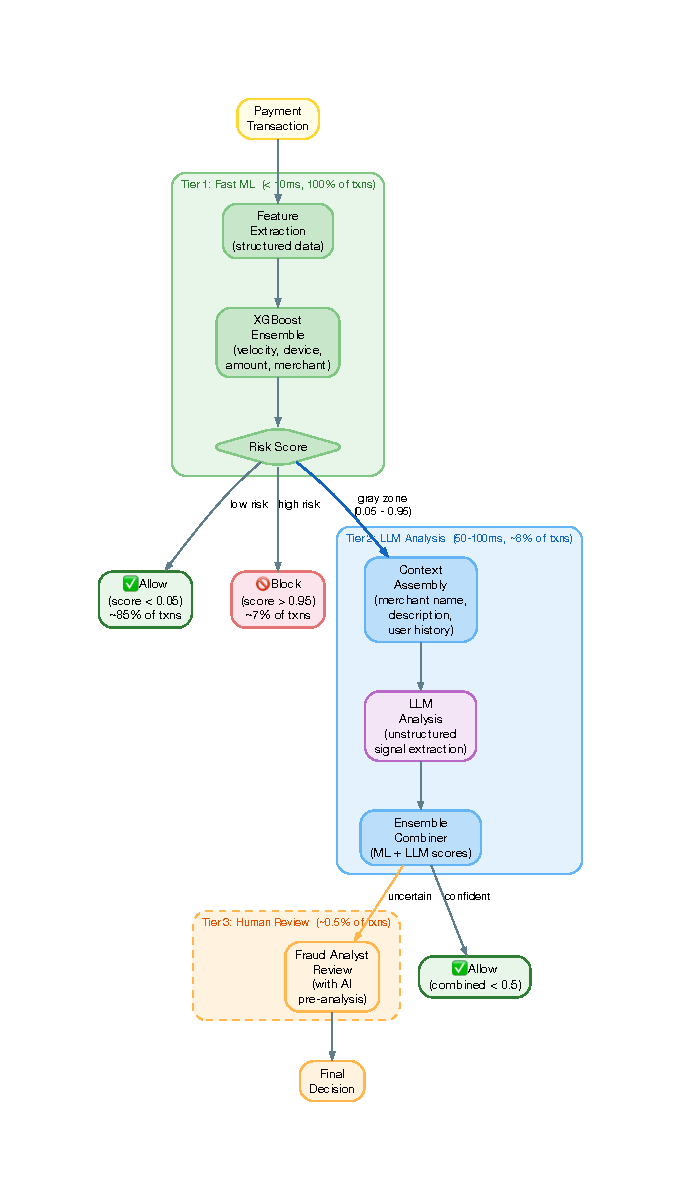
\includegraphics[width=\textwidth]{diagrams/compiled/ch06/stripe-hybrid-fraud.pdf}
\caption{Stripe's tiered fraud detection: fast ML handles 92\% of transactions, LLM analyzes the gray zone, humans review edge cases}
\label{fig:stripe-fraud}
\end{figure}


Stripe's API documentation is famously well-written, but their developer support team still handled thousands of questions daily. They built an internal documentation agent that:

\begin{enumerate}[leftmargin=*]
    \item Indexes all API documentation, changelogs, and internal knowledge base articles using a RAG pipeline
    \item Understands the user's specific integration context (which API version, which language SDK, what Stripe products they use)
    \item Generates code examples tailored to the user's stack, not generic examples
    \item Routes complex questions to human support engineers with full context
\end{enumerate}

The result: 65\% of support queries were resolved without human intervention, and the average resolution time for the remaining 35\% dropped by 40\% because human agents received pre-analyzed context.

\section{LinkedIn: Content Moderation at Billion-User Scale}

LinkedIn moderates hundreds of millions of posts, comments, and messages daily. Their LLM-based moderation system illustrates the challenges of deploying LLMs at true internet scale.

\subsection{The Tiered Moderation Architecture}

\begin{lstlisting}[language=Python, caption={LinkedIn's tiered moderation architecture}]
class ContentModerator:
    """
    Three-tier moderation: fast classifiers catch the obvious,
    LLMs handle the subtle, humans handle the ambiguous.
    """
    def moderate(self, content: UserContent) -> ModerationResult:
        # Tier 1: Fast classifiers (< 5ms, handles ~92% of content)
        # Regex, keyword lists, small fine-tuned BERT models
        fast_result = self.fast_classifier.predict(content)
        if fast_result.confidence > 0.95:
            return fast_result
        
        # Tier 2: LLM analysis (50-200ms, handles ~7% of content)
        # For content that fast classifiers are unsure about:
        # sarcasm, coded language, context-dependent violations
        llm_result = self.llm_moderator.analyze(
            content=content,
            user_history=self.get_user_context(content.author_id),
            thread_context=self.get_thread(content.parent_id),
        )
        if llm_result.confidence > 0.85:
            return llm_result
        
        # Tier 3: Human review (hours, handles ~1% of content)
        # LLM provides a pre-analysis brief for the human reviewer
        return self.escalate_to_human(
            content=content,
            ai_analysis=llm_result,
            similar_past_decisions=self.case_db.search(content, k=5),
        )
\end{lstlisting}

Key insight: the LLM handles only 7\% of content, but it's the \emph{hardest} 7\%---the content where context matters, where sarcasm might be confused with hate speech, where a post about ``shooting'' might be about basketball or photography. This is exactly where LLMs add the most value: the gray area between obviously fine and obviously problematic.

\subsection{Cost Engineering}

At LinkedIn's scale, even small per-request costs compound dramatically. Their cost engineering approach:

\begin{itemize}[leftmargin=*]
    \item \textbf{Cascade architecture}: Only 7\% of content reaches the LLM tier, keeping costs manageable
    \item \textbf{Prompt caching}: Similar content patterns (spam campaigns, coordinated abuse) share cached LLM analyses
    \item \textbf{Batch processing}: Non-urgent moderation (e.g., profile bios) is batched and processed during off-peak hours at lower cost
    \item \textbf{Self-hosted models}: For the highest-volume patterns, they fine-tuned smaller models (7B) that run on their own GPU infrastructure at a fraction of API costs
\end{itemize}

\section{Uber: The Centralized GenAI Gateway}

Uber operates thousands of microservices, and by 2024, hundreds of teams wanted to use LLMs. Without coordination, this would have resulted in hundreds of independent integrations---each with its own error handling, logging, and billing. Their solution: a centralized \textbf{GenAI Gateway} built by the Michelangelo team.

\begin{figure}[htbp]
\centering
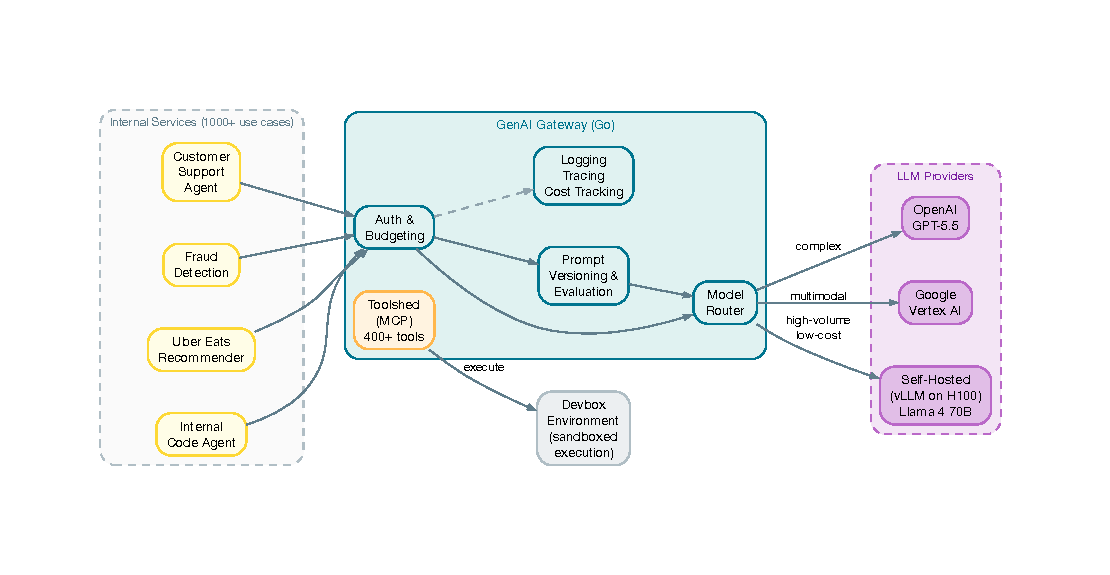
\includegraphics[width=\textwidth]{diagrams/compiled/ch06/uber-genai-gateway.pdf}
\caption{Uber's GenAI Gateway: a single infrastructure layer that abstracts multiple LLM providers and provides observability, auth, and cost tracking}
\label{fig:uber-gateway}
\end{figure}

Key architectural decisions:

\begin{itemize}[leftmargin=*]
    \item \textbf{Go-based gateway}: Written in Go for low-latency proxying, the gateway wraps third-party clients behind a unified API. Teams use familiar OpenAI-style APIs while the gateway handles routing, retries, and failover
    \item \textbf{MCP-based tooling (``Toolshed'')}: Over 400 internal tools exposed through the Model Context Protocol, carefully scoped per use case to avoid context window bloat
    \item \textbf{LangEffect framework}: An opinionated wrapper over LangGraph that enforces deterministic gates between LLM reasoning steps---linters, unit tests, and validation checks that the agent cannot skip
    \item \textbf{Zero-trust identity}: Every agent has a cryptographic identity tied to Uber's zero-trust architecture, providing full accountability for ``who did what, when, and why''
\end{itemize}

The result: teams can go from idea to production LLM feature in days instead of months, while the platform team maintains centralized observability, cost tracking, and security review.

\section{Patterns Across Enterprise Deployments}


Across all four case studies, we see recurring patterns:

\begin{table}[htbp]
\centering
\caption{Common patterns in enterprise LLM deployments}
\label{tab:enterprise-patterns}
\begin{tabularx}{\textwidth}{lX}
\toprule
\textbf{Pattern} & \textbf{Description} \\
\midrule
Tiered architecture & Use the cheapest/fastest model first; escalate to more powerful (and expensive) models only for difficult cases \\
Hybrid ML + LLM & Combine traditional ML (fast, cheap, interpretable) with LLMs (flexible, contextual) rather than replacing one with the other \\
Human-in-the-loop & LLMs handle the easy and medium cases; humans handle edge cases and provide training signal \\
Metric-driven deployment & Define acceptance criteria before deployment; measure relentlessly; roll back when quality degrades \\
Context is king & Investing in context assembly (RAG, user history, related data) yields better ROI than upgrading to a larger model \\
\bottomrule
\end{tabularx}
\end{table}

\section{Chapter Summary}

\noindent
Enterprise LLM deployment is 20\% model selection and 80\% systems engineering. The organizations that succeed:

\begin{enumerate}[leftmargin=*]
    \item Start with a clear problem and a measurable success metric---not ``we should use AI''
    \item Use the cheapest model that meets their quality bar, not the most powerful one available
    \item Build tiered architectures that reserve expensive LLM calls for cases where they add the most value
    \item Invest heavily in context assembly and evaluation infrastructure
    \item Plan for failure: graceful degradation, fallback paths, and human escalation
\end{enumerate}

\begin{keytakeaway}
The pattern across every successful enterprise AI deployment is the same: start narrow, measure relentlessly, and invest more in the engineering around the model than in the model itself. The companies that treat AI as a ``drop-in API call'' fail. The companies that treat it as a systems engineering challenge succeed.
\end{keytakeaway}
